\documentclass[11,leqno,fleqn]{scrbook}

\usepackage[utf8]{inputenc}
\usepackage[german]{babel}
\usepackage{amsmath}
\usepackage{amsthm}

\usepackage{pxfonts}
\newcommand{\N}{\mathbb{N}}
\newcommand{\Z}{\mathbb{Z}}
\newcommand{\Q}{\mathbb{Q}}
\newcommand{\R}{\mathbb{R}}

\newcommand{\kgV}[2]{
	\mathrm{kgV}(#1; #2)
}
\newcommand{\ggT}[2]{
	\mathrm{ggT}(#1; #2)
}

\usepackage{float}
\usepackage{graphicx}
\usepackage{tabularx}

\usepackage{tikz}
\usepackage{hyperref}
\usepackage{wrapfig}
\graphicspath{{figures/}}

\usepackage{tcolorbox}
\newtcolorbox{defn}[2][]{colback=green!10!white,
colframe=green!70!black,
width=.9\linewidth,
before=\par\smallskip\centering,
after=\par,
title=#2,
#1}

\newtcolorbox{law}[2][]{colback=red!10!white,
colframe=red!70!black,
width=.97\linewidth,
before=\par\smallskip\centering,
after=\par,
title=#2,
#1}

\setlength{\parindent}{0mm}

\newtheoremstyle{DefinitionsAndTheorems}{7pt}{3pt}{}{}{\bfseries}{}{\newline}{\thmname{#1} \thmnumber{#2}: \thmnote{#3.}}
\theoremstyle{DefinitionsAndTheorems}
\newtheorem{definition}{Definition}[section]
\newtheorem{theorem}{Satz}[section]

\newtheoremstyle{ExamplesAndExercises}{7pt}{3pt}{}{}{\bfseries}{}{ }{\thmname{#1} \thmnumber{#2} \thmnote{(#3)}}
\theoremstyle{ExamplesAndExercises}
\newtheorem{xmpl}{Beispiel}[chapter] % Dies wird unten mit newenvironment umgedeutet zwecks Kreis als Schlusssymbol
\newtheorem{exercise}{Übung}[section]

% Siehe newtheorem xmpl ohne Kreis als Schlusssymbol
\newenvironment{example}[1]{\begin{xmpl}#1}{\hfill $^\bigcirc$ \end{xmpl}}

% Beweis-Umgebung mit q.e.d.-Box und ohne Eingabe von "Beweis"; heisst prove, da proof reserviert;
\newenvironment{prove}{\begin{proof}[Beweis]}{\end{proof}}

% Lernzielumgebung
\newenvironment{lernziele}{\subsubsection*{Lernziele}\begin{itemize}}{\end{itemize}}

\newcommand{\rowheight}{\parbox[c][.7cm][s]{0.1cm}{~}}
\newcommand{\relationBox}{~\fbox{\color{white} AA\rowheight}~}

%***********
%\includeonly{}
%***********

\title{Mathematik I}
\author{\copyright Mathias Bosshardt und Franziska Flegel}
\date{Herbst 2024}

\begin{document}
\maketitle

\frontmatter
\tableofcontents  %\listoftables  \listoffigures

\mainmatter
\chapter{Einführung}

\section{Was ist Mathematik?}
\begin{wrapfigure}{r}{0.45\textwidth}
    \vspace{-.8cm}
	\begin{center}
		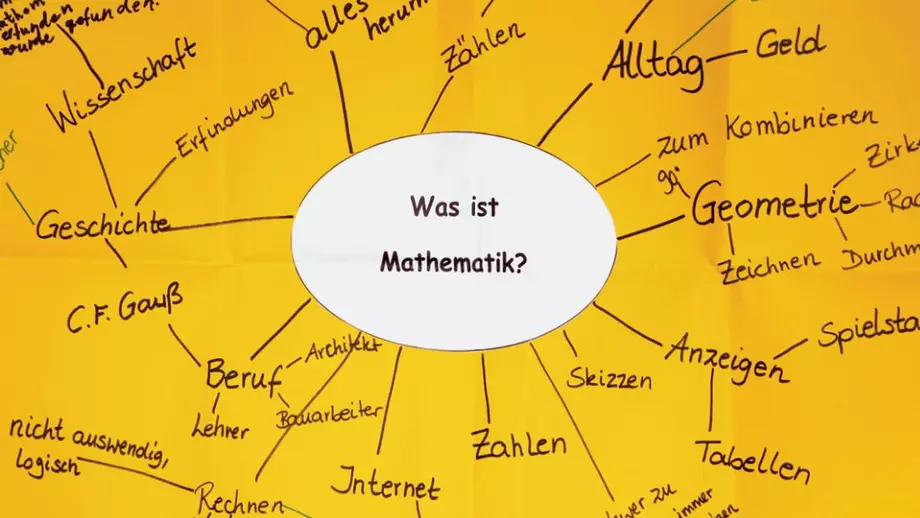
\includegraphics[width=0.96\linewidth]{WasIstMathematik}
	\end{center}
\end{wrapfigure}
Mathematik ist keine Naturwissenschaft. Sie hat aber dennoch viele Anwendungen in den Naturwissenschaften, insbesondere in der Physik, aber auch in anderen Disziplinen, wie etwa den Ingenieur- oder Wirtschaftswissenschaften.
Mathematik beschäftigt sich damit, Muster und Strukturen zu erkennen. 
Sie vermittelt keine interpretationsbedürftigen Ansichten.
Sie baut auf objektiven Sachverhalten und logischen Schlussfolgerungen auf.\par

\section{Warum Mathematik?}
Durch Mathematik können wir viele Dinge in der Welt besser verstehen und begründete Zukunftsprognosen abgeben.
Mathematik ist ein Teil unserer Kultur und zugleich die Antwort des Menschen auf die Komplexität der Welt.
Uns ist oft nicht bewusst, wie
\begin{wrapfigure}{l}{0.5\textwidth}
    \vspace{-.4cm}
	\begin{center}
		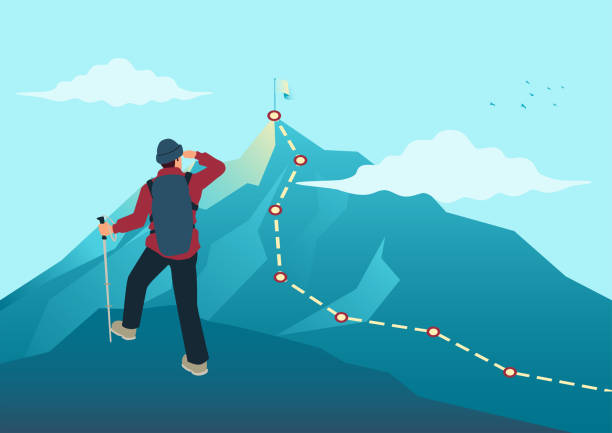
\includegraphics[width=0.96\linewidth]{Bergsteigen}
	\end{center}
	\caption{Der Weg ist das Ziel.}
\end{wrapfigure}
sehr unser Alltag mit Mathematik durchsetzt ist.
Mathematik steckt im Mobiltelefon, im Auto, in stabilen Gebäuden, in medizinischen Untersuchungsmethoden, in CDs, in der kühlen Cola, die du trinkst, wenn es dir mal wieder zu heiss wird\ldots
Mathematisches Können erwirbt man aber nur durch mathematisches Tun. Wer in der Mathematik voran kommen will, muss üben, sich mit der Materie auseinandersetzen. Bergsteigen lernt man ja auch nicht, indem man Bücher über Berge liest.
Wer die Aussicht auf dem Gipfel geniessen will, muss sich anstrengen, muss sich der Aufgabe stellen und selber auf den Berg steigen.
Genauso lassen sich die Schönheit und Harmonie der Mathematik nur erkennen, wenn man sich mit ihr beschäftigt.

\begin{figure}
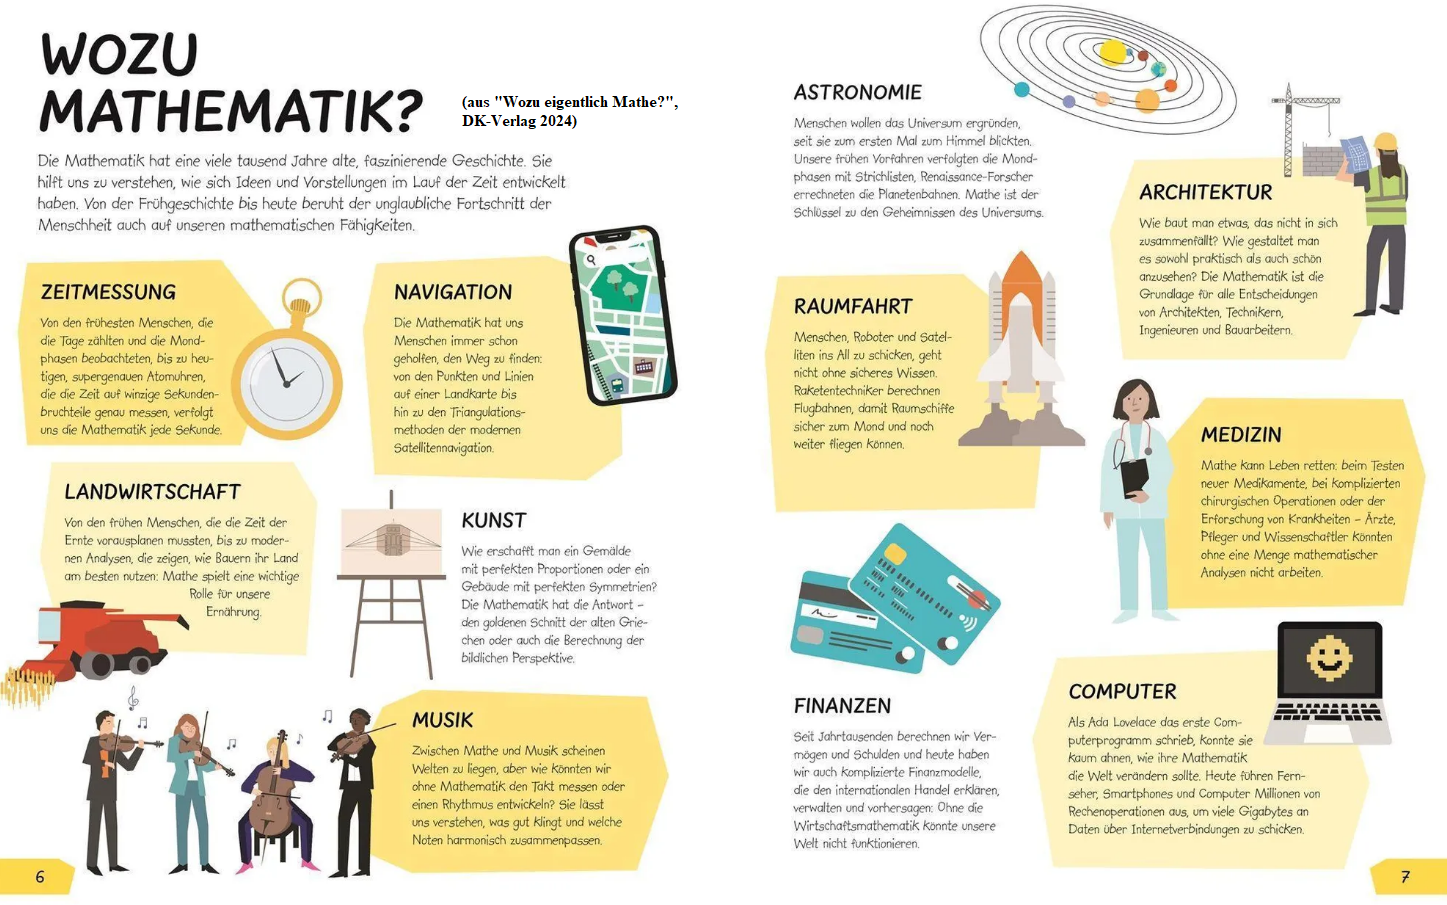
\includegraphics[angle=90,scale=0.6]{WozuMathematik}
\end{figure}
\thispagestyle{empty}

\chapter{Brückenkapitel (0)}
Im ersten Kapitel, oder eher im nullten gemäss Aufgabenbuch, repetieren wir einige Dinge, die ihr auf der Oberstufe gelernt habt.
Damit sind wir dann alle auf dem gleichen Stand.
Und teilweise erweitern wir unser Wissen bereits etwas, führen vielleicht neue Schreibweisen ein, formulieren die Rechengesetze evtl. etwas allgemeiner oder manchmal abstrakter, als du es bisher gewohnt warst. Vielleicht ist das für dich zum grössten Teil ein alter Hut - aber Übung macht den Meister!

\section{Rechnen mit Zahlen -- Die Rechengesetze}
Ein Gesetz ist bekanntermaßen eine feste Regel oder eine verbindliche Vorschrift.
An ihm darf man nichts rütteln oder verschieben, sondern man muss sich daran halten.
Genauso, wie es in den Gesetzbüchern Gesetze gibt, gibt es auch in der Mathematik Regeln, die gelten und beim Rechnen eingehalten werden müssen.
Diese sind die Rechengesetze oder Rechenregeln.
\begin{center}
\begin{tcolorbox}[colback=green!10!white,colframe=green!70!black,title=Rechengesetz,width=.9\linewidth]
		Ein Rechengesetz ist eine verbindliche Rechenvorschrift.
\end{tcolorbox}
\end{center}
Wenn du ein Rechengesetz missachtest, bekommst du natürlich keine Strafe von der Polizei.
Aber wenn du dich nicht an die Rechengesetze hältst, dann wird dein Ergebnis mit grosser Wahrscheinlichkeit falsch sein.
Die Rechengesetze gibt es also nicht, um verzweifelte Schüler:innen zu quälen, sondern sie ergeben mathematisch und logisch Sinn.

Wenn man von den Rechengesetzen spricht, dann meint man meistens das Assoziativgesetz, das Kommutativgesetz und das Distributivgesetz.
Sie sind die drei wichtigsten Rechengesetze.Wenn man den Begriff aber etwas weiter fasst, gibt es noch einige weitere Rechenregeln.
Diese sind etwa die Regel Punkt-vor-Strich, die Potenzgesetze und die Wurzelgesetze, oder Vorgehensweisen zum Auflösen von Klammern.
Fangen wir also an.

\subsection{Rechengesetze}

\begin{center}
\begin{tcolorbox}[colback=red!10!white,colframe=red!70!black,title=Rechengesetze,width=.97\linewidth]
	\begin{enumerate}
        \item
			Kommen Potenzen vor, müssen diese als erstes berechnet werden.
		\item
			Klammern in Termen müssen zuerst aufgelöst werden. ("`von innen nach aussen"')
        \item
			Punktrechnungen ( $\cdot$ und : ) müssen vor Strichrechnungen ( + und -- ) ausgeführt werden.
		\item
			Assoziativgesetz der Addition:\\
			Für alle rellen Zahlen $a$, $b$ und $c$ gilt: $(a+b)+c = a+(b+c)$
		\item
			Assoziativgesetz der Multiplikation:\\
			Für alle rellen Zahlen $a$, $b$ und $c$ gilt: $(a\cdot b)\cdot c = a\cdot (b\cdot c)$
		\item
			Kommutativgesetz der Addition:\\
			Für alle rellen Zahlen $a$ und $b$ gilt: $a+ b= b+ a$
		\item
			Kommutativgesetz der Multiplikation:\\
			Für alle rellen Zahlen $a$ und $b$ gilt: $a\cdot b= b\cdot a$
		\item
			Distributivgesetz der Multiplikation:\\
			Für alle rellen Zahlen $a$, $b$ und $c$ gilt: $(a\pm b)\cdot c = a\cdot c \pm b\cdot c$
		\item
			Distributivgesetz der Division:\\
			Für alle rellen Zahlen $a$, $b$ und $c$ gilt: $(a\pm b): c = a: c \pm b: c$	
	\end{enumerate}
\end{tcolorbox}
\end{center}

\begin{example}
Im folgenden Term darf nicht einfach von links nach rechts gerechnet werden, sondern es muss zuerst das Produkt berechnet werden:
\[
	5+5\cdot 3
\]
\end{example}

\begin{example}
Berechne den folgenden Term:
\[
	4\cdot(27-(3\cdot (5+3)+2))
\]
\end{example}

\begin{example}
Rechne vorteilhaft:
\[
	85+33+67
\]
\end{example}

\begin{example}
Rechne vorteilhaft:
\[
	7\cdot 4 \cdot 45
\]
\end{example}

\begin{example}
Ebenso:
\[
	24+33+76
\]
\end{example}

\begin{example}
Multipliziere aus:
\[
	4\cdot (20-5)
\]
\end{example}

\begin{example}
Manchmal bringt ausklammern einen Vorteil!
\[
	14\cdot 13 - 4\cdot 13
\]
\end{example}

\begin{tcolorbox}[colback=green!10!white,colframe=green!70!black,title=Betrag einer Zahl,width=.9\linewidth]
		Für eine Zahl $a$ ist der Betrag der Zahl
		\[
			|a|=\left\{\begin{array}{ll} a, & a\ge 0 \\
         -a, & a<0\end{array}\right.
		\]
\end{tcolorbox}


\section{Terme}
\subsection*{Auswerten}
Mit $T(a,b)$ bezeichnen wir einen Term, der die Variablen $a$ und $b$ enthält. Setzt man anstelle von $a$ und $b$ Zahlen ein, z.B. 5 für $a$ und 3 für $b$, so schreiben wir $T(5,3)$.
\vspace{1cm}

\subsection*{Termumformungen}
Zwei Terme $T_1$ und $T_2$ heissen \emph{äquivalent (gleichwertig)}, wenn alle möglichen Einsetzungen für die Variable(n) bei $T_1$ denselben Wert ergeben wie bei $T_2$.
Man schreibt: $T_1 = T_2$.
\vspace{5mm}
Einen Term umformen bedeutet:
Man ersetzt ihn durch einen äquivalenten Term. Beim Umformen von Termen werden die arithmetischen Grundgesetze gebraucht.

\begin{tcolorbox}[colback=red!7!white,colframe=red!60!black,title=Arithmetische Grundgesetze]
    \bgroup
    \def\arraystretch{2.5}
	\begin{tabularx}{\linewidth}{|X|c|c|}
			\hline
			 & Addition & Multiplikation \\
			\hline
			Kommutativgesetz & $a+b=b+a$ & $a\cdot b = b\cdot a$ \\
			
			Assoziativgesetz & $(a+b)+c = a+ (b+c)$ & $(a\cdot b)\cdot c = a\cdot (b\cdot c)$ \\
			
			Neutralelement 0 bzw. 1 & $a+0 = a$ & $a\cdot 1 = a$ \\
			
			Inverses Element $-a$ bzw. $\displaystyle \frac{1}{a}$ & $a+(-a) = 0$ & $\displaystyle a\cdot \frac{1}{a} = 1$ \\
			\hline
			Distributivgesetz & \multicolumn{2}{c|}{$a(b+c)=ab+ac$} \\
			\hline
    \end{tabularx}
    \egroup
\end{tcolorbox}

\subsection*{Formeln}
Die \emph{Binomischen Formeln} benutzt man zum schnellen Umformen von Produkten aus Binomen.
Sie stellen Merkformeln dar, die einerseits das Ausmultiplizieren von Klammerausdrücken erleichtern, andererseits aber auch die Faktorisierung von Termen (Umformung von bestimmten Summen und Differenzen in Produkte) erlauben.

\begin{tcolorbox}[colback=blue!7!white,colframe=blue!60!black,title=Binomische Formeln]
	\begin{tabbing}
		$(a+b)^2$ \qquad \, \, \= $=$ \, \= $a^2+2ab+b^2$ \\
		$(a-b)^2$ \qquad \, \, \= $=$ \, \= $a^2-2ab+b^2$ \\
		$(a+b)(a-b)$ \> $=$ \> $a^2-b^2$
	\end{tabbing}
\end{tcolorbox} 

Es gibt auch trinomische Formeln: $(a+b+c)^2$. Kannst du dafür auch einen Ausdruck angeben?
\vspace{2cm}

\subsection*{Erweiterung}
Mit dem \emph{Pascalschen Dreieck} kann man auch höhere Potenzen von Binomen schnell ausmultiplizieren:
\[
	(a+b)^3 =
\]






\chapter{Zahlenbereiche}
\section{Natürliche Zahlen}
Die natürlichen Zahlen 1, 2, 3, 4, \ldots ~sind die ältesten Zahlen, die sich aus dem Zählen von Gegenständen entwickelt haben.
Dabei nimmt man an, dass man immer weiterzählen kann.\\

\begin{defn}{Natürliche Zahlen}
	Die Menge der natürlichen Zahlen wird mit $\N$ bezeichnet.
	Man schreibt:
	\begin{align*} 
	 \N = \{ 1, 2, 3, 4, \ldots \}\, .
	\end{align*}
	Die Zahlen $1, 2, 3, 4, \ldots$ heissen \emph{Elemente} der Menge $\N$.
	Ist eine Zahl $n$ eine natürliche Zahl, so schreibt man: $n\in\N$\,.
\end{defn}

\vspace{.5cm}
\begin{wrapfigure}{r}{6cm}
	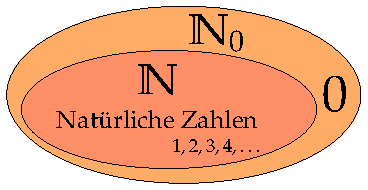
\includegraphics[width=\linewidth]{numberset-naturals-N0}
\end{wrapfigure}
Das Zeichen \glqq $\in$\grqq~bedeutet: \glqq ist Element von\grqq, das Zeichen \glqq $\notin$\grqq~bedeutet: \glqq ist \emph{nicht} Element von\grqq.

\paragraph{Achtung!}
Die Zahl 0 wird dabei {\bfseries nicht} mit dazu genommen.
Wir schreiben:
\begin{align*}
  0 \notin \N\, .
\end{align*}
Möchte man die Null mit einschliessen, so verwenden wir die Schreibweise $\N_0$.\\

\begin{defn}{Natürliche Zahlen zusammen mit Null}
	Die Menge der natürlichen Zahlen wird mit $\N_0$ bezeichnet.
	Man schreibt: $\N_0 = \{ 0, 1, 2, 3, 4, \ldots \}$\,.
\end{defn}

\begin{example}
  Schreibe in das Symbol \relationBox das richtige Zeichen $\in$ oder $\notin$ hinein.
  \begin{align*}
   2 \relationBox \N_0\,,\qquad
   \frac{1}{2} \relationBox \N\,,\qquad
   0 \relationBox \N\,,\qquad
   0 \relationBox \N_0\,,\qquad
   \frac{72}{36} \relationBox \N\,.
  \end{align*}

\end{example}


\vspace{.5cm}
Die natürlichen Zahlen braucht man z.B. um Anzahlen anzugeben, Rangplätze oder Reihenfolgen festzulegen oder (bestimmte) Messergebnisse festzuhalten.

\begin{example}~
	\begin{itemize}\setlength\itemsep{0pt}
		\item Wir haben heute 6 Lektionen. (Anzahl)
		\item Heute ist der erste Tag des Monats. (Rangplatz)
		\item Heute ist es 30 Grad warm. (Messergebnis)
	\end{itemize}
\end{example}

Man kann mit den natürlichen Zahlen auch (bestimmte) Gleichungen lösen.
\begin{example}
 Heute ist es \unit[30]{°C} warm und damit \unit[2]{°C} wärmer als gestern.
 D.h. für die Temperatur $x$ von gestern in \unit{°C} gilt die Gleichung:
 \begin{align*}
   x + 2 = 30
 \end{align*}
Die Lösung der Gleichung ist eine natürliche Zahl, nämlich $x = 28$\,, d.h. die gesuchte Temperatur ist \unit[28]{°C}
\end{example}


\section{Negative ganze Zahlen}
\begin{wrapfigure}{r}[1cm]{5cm}
 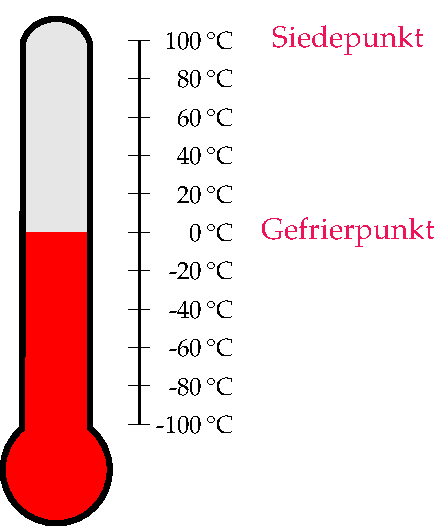
\includegraphics[width=\linewidth]{thermometer}
\end{wrapfigure}
Für viele Zwecke reichen die natürlichen Zahlen nicht aus.
Ist es heute z.B. \unit[30]{°C} warm und wir wollen es mit der Temperatur vor einem halben Jahr vergleichen, so stellen wir vielleicht fest, dass es heute \unit[35]{°C} wärmer ist als vor einem halben Jahr.
D.h. die Temperatur $x$ vor einem halben Jahr in \unit{°C} erfüllt die Gleichung:
\begin{align*}
	x + 35 = 30
\end{align*}
Diese Gleichung lässt sich nicht mit den natürlichen Zahlen lösen, wohl aber, wenn wir negative Zahlen zulassen.
Dann erhalten wir: $x = -5$\,, d.h. die Temperatur ist \unit[--5]{°C}\,.

\subsection{Weitere Beispiele}
Die folgenden Beispiele zeigen, dass im Alltag negative Zahlen oft in Verbindung mit einer künstlich festgelegten Null vorkommen.

\paragraph{Temperatur.}
In Europa misst man die Temperatur in \unit{°C}.
Diese Temperaturskala ist so definiert, dass bei Normaldruck der Gefrierpunkt des Wasser gleich \unit[0]{°C} entspricht und der Siedepunkt gleich \unit[100]{°C}.
Wenn eine Temperatur also unter der Temperatur des Wassergefrierpunkts ist, so ist sie negativ.

\paragraph{Meter über dem Meeresspiegel.}
Auf Landkarten wird die Höhe z.B. in Metern über dem Meeresspiegel (m ü.M.) angegeben.
Zum Beispiel liegt der Gipfel des Mt. Whitney in den USA \unit[4418]{m} über dem Meer, kurz \unit[4418]{m ü.M.}
Dabei wurde der Meeresspiegel künstlich als \emph{Normalhöhe} festgelegt.
Dies führt dazu, dass das sogenannte \emph{Tal des Todes} sich bei \unit[-86]{m ü.M.} befindet.

\subsection{Zahlengerade}
\begin{figure}[H]
	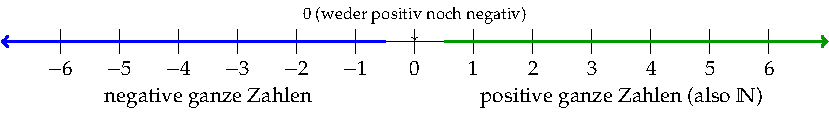
\includegraphics[width=\linewidth]{zahlengerade}
	\caption{Die Zahlengerade mit den positiven ganzen Zahlen rechts von der Null und den negativen ganzen Zahlen links von der Null.
	Die Null ist weder positiv noch negativ.}
	\label{fig:zahlengerade-pos-neg}
\end{figure}

Die sogenannten negativen ganzen Zahlen $-1, -2, -3, \ldots$ stehen links von 0 auf der Zahlengeraden, siehe Abbildung \ref{fig:zahlengerade-pos-neg}.
Die natürlichen Zahlen, die auch positive ganze Zahlen genannt werden, stehen rechts von Null auf der Zahlengeraden. Beachte, dass die Null selbst weder positiv noch negativ ist.
Möchtest du die Zahlen in $\N_0$ auf diese Weise bezeichnen (also die Null mit einschliessen), so kannst du sie nicht-negative ganze Zahlen nennen.

\section{Ganze Zahlen}
\begin{wrapfigure}{r}{7cm}
	\vspace{-1cm}
	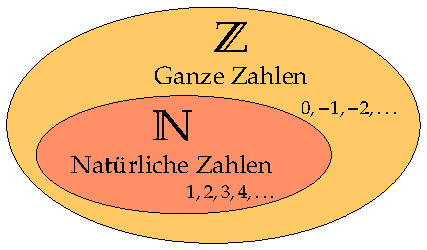
\includegraphics[width=\linewidth]{numberset-integers}
	% \caption{Die natürlichen Zahlen sind in den ganzen Zahlen enthalten.
	% Auf eine Darstellung der Menge $\N_0$ wurde hier für die bessere Übersicht verzichtet.}
	% \label{fig:numberset-integers}
	\vspace{-2cm}
\end{wrapfigure}
Die Menge der ganzen Zahlen besteht aus den natürlichen Zahlen, den negativen ganzen Zahlen und der Null.

Jede natürliche Zahl ist auch eine ganze Zahl, aber nicht andersherum.
D.h. die Menge der natürlichen Zahlen ist komplett in der Menge der ganzen Zahlen enthalten.
%, siehe Abbildung \ref{fig:numberset-integers}.

\vspace{1cm}
\begin{defn}{Ganzen Zahlen}
	Fügt man zu den natürlichen Zahlen $\N$ die Zahl 0 und die negativen ganzen Zahlen $-1, -2, -3,\ldots$ hinzu,
	so erhält man die Menge der ganzen Zahlen $\Z = \{ \ldots, -3, -2, -1, 0, 1, 2, 3, \ldots \}$\, .
\end{defn}


\subsection{Regeln}
Für das Rechnen mit den ganzen Zahlen gelten die arithmetischen Grundgesetze von Seite \pageref{law:arithmetic}, bis auf eine Ausnahme!
Welche? (Schreibe es selber auf.)\\
\kariert{15}{2}\\~\\
Vervollständige die Übersicht von Seite \pageref{law:arithmetic} für alle Regeln bis auf die, die nicht gilt:
\begin{law}{Arithmetische Grundgesetze für \underline{\bfseries die ganzen Zahlen}}
    \bgroup
    \def\arraystretch{2.5}
	\begin{tabularx}{\linewidth}{|X|p{3.7cm}|p{3.7cm}|}
			\hline
			 & Addition & Multiplikation \\
			\hline
			Kommutativgesetz &  &  \\\hline
			Assoziativgesetz &  &  \\\hline
			Es gibt Neutralelement\newline 0 bzw. 1\,. &  &  \\\hline
			Es gibt inverses Element\newline~ & & \\
			\hline
			Distributivgesetz & \multicolumn{2}{c|}{} \\
			\hline
    \end{tabularx}
    \egroup
\end{law}

\subsection{Subtraktion}
Mithilfe der negativen Zahlen kann man die Subtraktion als eine Addition mit einer negativen Zahl schreiben und so die Rechenregeln, die für die Addition gelten, anwenden, wie z.B. das Kommutativgesetz und das Assoziativgesetz.
\begin{example} Kommutativgesetz der Addition:
	\begin{align*}
					8 - 5		&\,=\, 8 + (-5) \,=\, (-5) + 8\\
		\text{Aber:}\quad 8 - 5		&\,\neq\, 5 - 8
	\end{align*}
	Wende das Kommutativgesetz einmal nach dem gleichen Schema selbst an:\\
	\kariert[\large 10 -- 3 \,=\,]{15}{1.5}\\
\end{example}
\begin{example} Assoziativgesetz der Addition:
	\begin{align*}
					(8 - 5) - 1			&\,=\, \bigl(8 + (-5)\bigr) + (-1) \,=\, 8 + \bigl( (-5) + (-1)\bigr)\\
		\text{Aber:}\quad (8 - 5) - 1	&\,\neq\, 8 - (5 - 1)
	\end{align*}
	Wende das Assoziativgesetz einmal nach dem gleichen Schema selbst an:\\
	\kariert[\large (10 -- 3) -- 2 \,=\,]{15}{2}\\
\end{example}
\begin{example} Minusklammer:
	\begin{align*}
					1 -(8 - 5)			&\,=\, 1 + (-1)\cdot\bigl(8 + (-5)\bigr)\,=\, 1 + (-1)\cdot 8 + (-1)\cdot (-5) = 1 - 8 + 5\\
	\end{align*}
	Wende die Minusklammer einmal nach dem gleichen Schema selbst an:\\
	\kariert[\large 10 -- (3 -- 2) \,=\,]{15}{2}\\
\end{example}

\section{Rationale Zahlen}
\begin{defn}{Rationale Zahlen}
	Die Menge der rationalen Zahlen $\Q$ besteht aus allen Zahlen, die man als Bruch schreiben kann.
	\begin{align*}
		\Q = \left\{\left. \frac{p}{q} ~\right|~ p,q \in \Z;~ q \neq 0\, \right\}
	\end{align*}
	
\end{defn}


% \section{Kann man alle Zahlen als Bruch darstellen?}
% Hier muss noch etwas Geschichte hin.



\end{document} 
